\section*{\nr.2 \tittwo (25 Punkte)}
\begin{enumerate}
\item Sei 
\begin{equation}
  \psi(x) = \psi_0 e^{-\frac{x^2}{4\sigma^2}}
\end{equation}
es wird angenommen, dass $\psi_0,\sigma\in\mathbb{R}_+$.
\begin{enumerate}[(a)]
\item 
\begin{equation}
  \int \mathrm{d}x |\psi|^2=\psi_0^2\sqrt{2\pi}\sigma^2
\end{equation}
\item 
\begin{equation}
  \langle x\rangle=\int  x |\psi|^2 \mathrm{d}x = 0,
\end{equation}
da man über das Produkt einer geraden mit einer ungeraden Funktion integriert.
\item 
\begin{equation}
  \langle x^2\rangle=\int x^2|\psi|^2\mathrm{d}x = \sqrt{2 \pi}\psi_0^2 \sigma^3
\end{equation}
daraus folgt mit (b)
\begin{equation}
  \Delta x = \sqrt{\langle x^2\rangle-\langle x\rangle^2}=\sqrt{\langle x^2\rangle}=\psi \sqrt[4]{2 \pi} \sigma^{3/2}
\end{equation}
\item Es gilt 
\begin{align}
  \phi(p,t)&=\frac{1}{\sqrt{2 \pi \hbar}}\int_{-\infty}^{\infty}\psi_0 \exp\left(\frac{-x^2}{4\sigma^2}\right)\exp\left(-\frac{ipx}{\hbar}\right)\mathrm{d}x\\
  &=\sqrt{\frac{2 \sigma^2}{\hbar}}\psi_0\exp\left(-\frac{p^2\sigma^2}{\hbar^2}\right)
\end{align}
daraus folgt
\begin{equation}
  \langle p \rangle= \int p |\phi(p,t)|^2 \mathrm{d}p = 0
\end{equation}
da man wie in (b) über das Produkt einer geraden und einer ungeraden Funktion integriert.
\item 
\begin{align}
  \langle E \rangle =  \frac{\langle p^2 \rangle}{2m} &=\frac{1}{2m} \int p^2 |\phi|^2 \mathrm{d}p \\
  &= \frac{1}{2m} \sqrt{\frac{\pi}{2}}\frac{\hbar^2 \psi_0^2}{\sigma}
\end{align}
\item Aus (d) und (e) folgt
\begin{equation}
  \Delta p = \sqrt{\langle p^2 \rangle} = \frac{\hbar \psi_0} {\sqrt{\sigma}}\sqrt[4]{\frac{\pi}{2}}
\end{equation}
und damit 
\begin{equation}
  \Delta x \Delta p = \psi_0^2\sigma^3\sqrt{\pi}\hbar
\end{equation}
\end{enumerate}
\item Sei 
\begin{equation}
  \psi(x)=\frac{\psi_0}{\sqrt{x^2+\sigma^2}}
\end{equation}
es wird angenommen, dass $\psi_0,\sigma\in\mathbb{R}_+$.
\begin{enumerate}
\item 
\begin{equation}
  \int \mathrm{d}x \frac{\psi_0^2}{x^2+\sigma^2}=\frac{\psi_0^2 \pi}{\sigma^2}
\end{equation}
\item 
\begin{equation}
  \langle x \rangle = \int x|\psi(x)|^2 \mathrm{d}x=0,
\end{equation}
da über ein Produkt einer geraden mit einer ungeraden Funktion integriert wird.
\item 
\begin{align}
  \langle x^2 \rangle &= \int x^2 \frac{\psi_0^2}{x^2+\sigma^2}\\
  &=[\psi_0(x-\sigma \arctan (x/\sigma))]_{-\infty}^{\infty}\rightarrow \infty
\end{align}
dieses Integral divergiert.\\
Da $\langle x^2 \rangle$ divergiert und $\Delta x = \sqrt{\langle x^2 \rangle}$ divergiert auch $\Delta x$.
\item Es gilt auch hier
\begin{align}
  \phi(p,t)&=\frac{1}{\sqrt{2 \pi \hbar}}\int_{-\infty}^{\infty} \frac{\psi_0}{\sqrt{x^2+\sigma^2}}\exp\left(-\frac{ipx}{\hbar}\right)\mathrm{d}x \\
  &= \phi_0 \sqrt{\frac{2}{\pi \hbar}}J_0\left(\frac{p \sigma}{\hbar}\right)
\end{align}
wobei $J_0$ die Besselfunktion bezeichnet.\\
Damit folgt 
\begin{equation}
  \langle p \rangle = 0
\end{equation}
\item 
\begin{equation}
  \langle E \rangle = \frac{\langle p^2 \rangle}{2 m} = \frac{1}{2m} \frac{\phi_0 \sqrt{2 \pi} h^{5/2}}{\sigma^3}
\end{equation}
\item \begin{equation}
  \Delta p = \sqrt{\langle p^2 \rangle} = \sqrt{\frac{\phi_0 \sqrt{2 \pi} h^{5/2}}{\sigma^3}}
\end{equation}
Da $\Delta x$ divergiert und $\Delta p >0 $ divergiert auch das Produkt $\Delta x \Delta p$. 
\end{enumerate}
\item 
\begin{figure}[htbp]
\centering
% GNUPLOT: LaTeX picture with Postscript
\begingroup
  \makeatletter
  \providecommand\color[2][]{%
    \GenericError{(gnuplot) \space\space\space\@spaces}{%
      Package color not loaded in conjunction with
      terminal option `colourtext'%
    }{See the gnuplot documentation for explanation.%
    }{Either use 'blacktext' in gnuplot or load the package
      color.sty in LaTeX.}%
    \renewcommand\color[2][]{}%
  }%
  \providecommand\includegraphics[2][]{%
    \GenericError{(gnuplot) \space\space\space\@spaces}{%
      Package graphicx or graphics not loaded%
    }{See the gnuplot documentation for explanation.%
    }{The gnuplot epslatex terminal needs graphicx.sty or graphics.sty.}%
    \renewcommand\includegraphics[2][]{}%
  }%
  \providecommand\rotatebox[2]{#2}%
  \@ifundefined{ifGPcolor}{%
    \newif\ifGPcolor
    \GPcolorfalse
  }{}%
  \@ifundefined{ifGPblacktext}{%
    \newif\ifGPblacktext
    \GPblacktexttrue
  }{}%
  % define a \g@addto@macro without @ in the name:
  \let\gplgaddtomacro\g@addto@macro
  % define empty templates for all commands taking text:
  \gdef\gplbacktext{}%
  \gdef\gplfronttext{}%
  \makeatother
  \ifGPblacktext
    % no textcolor at all
    \def\colorrgb#1{}%
    \def\colorgray#1{}%
  \else
    % gray or color?
    \ifGPcolor
      \def\colorrgb#1{\color[rgb]{#1}}%
      \def\colorgray#1{\color[gray]{#1}}%
      \expandafter\def\csname LTw\endcsname{\color{white}}%
      \expandafter\def\csname LTb\endcsname{\color{black}}%
      \expandafter\def\csname LTa\endcsname{\color{black}}%
      \expandafter\def\csname LT0\endcsname{\color[rgb]{1,0,0}}%
      \expandafter\def\csname LT1\endcsname{\color[rgb]{0,1,0}}%
      \expandafter\def\csname LT2\endcsname{\color[rgb]{0,0,1}}%
      \expandafter\def\csname LT3\endcsname{\color[rgb]{1,0,1}}%
      \expandafter\def\csname LT4\endcsname{\color[rgb]{0,1,1}}%
      \expandafter\def\csname LT5\endcsname{\color[rgb]{1,1,0}}%
      \expandafter\def\csname LT6\endcsname{\color[rgb]{0,0,0}}%
      \expandafter\def\csname LT7\endcsname{\color[rgb]{1,0.3,0}}%
      \expandafter\def\csname LT8\endcsname{\color[rgb]{0.5,0.5,0.5}}%
    \else
      % gray
      \def\colorrgb#1{\color{black}}%
      \def\colorgray#1{\color[gray]{#1}}%
      \expandafter\def\csname LTw\endcsname{\color{white}}%
      \expandafter\def\csname LTb\endcsname{\color{black}}%
      \expandafter\def\csname LTa\endcsname{\color{black}}%
      \expandafter\def\csname LT0\endcsname{\color{black}}%
      \expandafter\def\csname LT1\endcsname{\color{black}}%
      \expandafter\def\csname LT2\endcsname{\color{black}}%
      \expandafter\def\csname LT3\endcsname{\color{black}}%
      \expandafter\def\csname LT4\endcsname{\color{black}}%
      \expandafter\def\csname LT5\endcsname{\color{black}}%
      \expandafter\def\csname LT6\endcsname{\color{black}}%
      \expandafter\def\csname LT7\endcsname{\color{black}}%
      \expandafter\def\csname LT8\endcsname{\color{black}}%
    \fi
  \fi
    \setlength{\unitlength}{0.0500bp}%
    \ifx\gptboxheight\undefined%
      \newlength{\gptboxheight}%
      \newlength{\gptboxwidth}%
      \newsavebox{\gptboxtext}%
    \fi%
    \setlength{\fboxrule}{0.5pt}%
    \setlength{\fboxsep}{1pt}%
\begin{picture}(7200.00,5040.00)%
    \gplgaddtomacro\gplbacktext{%
      \csname LTb\endcsname%
      \put(814,704){\makebox(0,0)[r]{\strut{}$0$}}%
      \put(814,1444){\makebox(0,0)[r]{\strut{}$0.2$}}%
      \put(814,2184){\makebox(0,0)[r]{\strut{}$0.4$}}%
      \put(814,2925){\makebox(0,0)[r]{\strut{}$0.6$}}%
      \put(814,3665){\makebox(0,0)[r]{\strut{}$0.8$}}%
      \put(814,4405){\makebox(0,0)[r]{\strut{}$1$}}%
      \put(946,484){\makebox(0,0){\strut{}$-10$}}%
      \put(2410,484){\makebox(0,0){\strut{}$-5$}}%
      \put(3875,484){\makebox(0,0){\strut{}$0$}}%
      \put(5339,484){\makebox(0,0){\strut{}$5$}}%
      \put(6803,484){\makebox(0,0){\strut{}$10$}}%
    }%
    \gplgaddtomacro\gplfronttext{%
      \csname LTb\endcsname%
      \put(176,2739){\rotatebox{-270}{\makebox(0,0){\strut{}$|\psi|^2$}}}%
      \put(3874,154){\makebox(0,0){\strut{}$x$}}%
      \csname LTb\endcsname%
      \put(5816,4602){\makebox(0,0)[r]{\strut{}$ psi_1$}}%
      \csname LTb\endcsname%
      \put(5816,4382){\makebox(0,0)[r]{\strut{}$ psi_2$}}%
    }%
    \gplbacktext
    \put(0,0){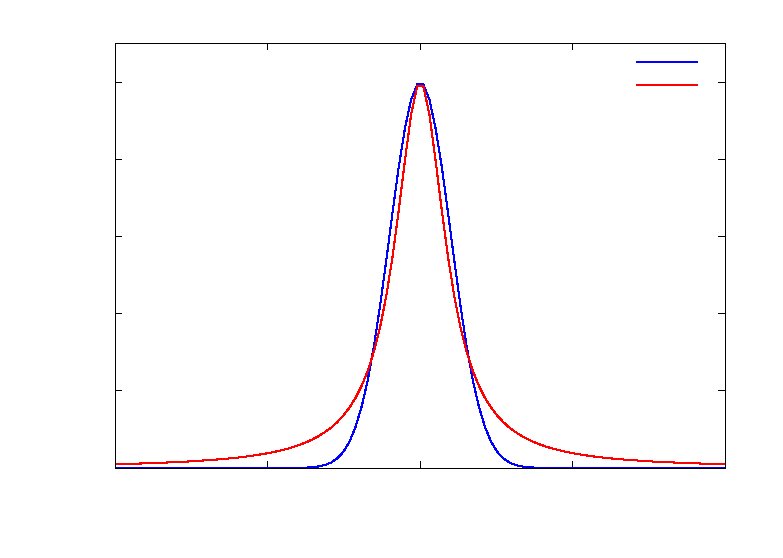
\includegraphics{plots}}%
    \gplfronttext
  \end{picture}%
\endgroup

\caption{Skizzen der Wellenfunktionen für $\psi_0=1$ und $\sigma=1$}
\label{fig:plots}
\end{figure}
Die erste Wellenfunktion kann ein quantenmechanisches Teilchen beschreiben, sofern $\phi_0$ udn $\sigma$ entsprechend gewählt werden. Die zweite Wellenfunktion verhält sich sehr anders als wir es von einem Teilchen erwarten würden, dass das Produkt aus Orts- und Impulsunschärfe divergiert ist eine sehr ungewöhnliche Eigenschaft. 
\end{enumerate}